\chapter{Theoretical background}\label{chap:lit}
\begin{overview} 
  This chapter explores existing developments in modelling and
  simulating steady-state and dynamic systems with and without
  uncertainty.
\end{overview}

\subsection{IEC 61131-3}
IEC 61131-3 is a standard that defines

\url{http://en.wikipedia.org/wiki/IEC_61131-3}

\section{Basic modelling equations}
Several equations are used in many different pieces of equipment
\subsection{Conservation of mass}
\subsection{Conservation of energy}
\subsection{Reaction kinetics}
\subsection{Equilibrium}
\subsection{Transport equations}
\subsubsection{Heat transfer}
\subsubsection{Mass transfer}

\section{Simulation}

\subsection{Modelling}
\subsubsection{Microscopic}

\subsubsection{Macroscopic}
Macroscopic modelling 

\subsubsection{Lumped models}

\subsection{Proprietary chemical systems}

\subsection{Modelica}
The Modelica project was spearheaded by \xxx, who started research on
modelling languages during his PhD studies in \xxx.

\subsection{Stochastic simulation}

\subsection{Proprietary simulators}

\subsection{Input identification}
Stochastic simulation of systems, especially those using Monte Carlo
methods, require good input scenarios to generate good output data.
It is common to make use of Markov processes to generate realistic
inputs based on historic data.  However, identification of ``events''
within historic data can be troublesome.  Much work has been done on
identification of events or trends in data (\cite{Maurya2007Fault}
gives an overview of trend analysis techniques).  Reduction of process
signals to symbols representing qualitative event types rather than
quantitative data allows patterns to be found in events, or what
Cheung and Stephanopoulos \cite{Cheung1990Representation} refer to as
episodes.  In this seminal work, the authors define a formal language
in terms of the 7 primitives shown in
figure~\ref{fig:stephanopoulosprimitives}.

\begin{figure}[htbp]
  \centering
  \setlength{\unitlength}{0.7em}
  {\small
  \begin{picture}(8,8)
    \put(0,0){\line(1,0){8}}
    \put(0,0){\line(0,1){8}}
    \put(7,1){D}
    \put(4,4){$(+,-)$}
    \thicklines
    \qbezier(1,1)(2,7)(7,7)
  \end{picture}
  }
  {\small
  \begin{picture}(8,8)
    \put(0,0){\line(1,0){8}}
    \put(0,0){\line(0,1){8}}
    \put(7,1){B}
    \put(1,4){$(+,+)$}
    \thicklines
    \qbezier(1,1)(7,2)(7,7)
  \end{picture}
  }
  {\small
  \begin{picture}(8,8)
    \put(0,0){\line(1,0){8}}
    \put(0,0){\line(0,1){8}}
    \thicklines
    \qbezier(1,1)(2,2)(7,7)
    \put(7,1){C}
    \put(1,5){$(+,0)$}
  \end{picture}
  }
  {\small
  \begin{picture}(8,8)
    \put(0,0){\line(1,0){8}}
    \put(0,0){\line(0,1){8}}
    \thicklines
    \qbezier(1,7)(6,7)(6.7,1)
    \put(7,1){G}
    \put(1,4){$(-,-)$}
  \end{picture}
  }
  {\small
  \begin{picture}(8,8)
    \put(0,0){\line(1,0){8}}
    \put(0,0){\line(0,1){8}}
    \thicklines
    \qbezier(1,7)(2,2)(6.7,1)
    \put(7,1){E}
    \put(4,4){$(-,+)$}
  \end{picture}
  }
  {\small
  \begin{picture}(8,8)
    \put(0,0){\line(1,0){8}}
    \put(0,0){\line(0,1){8}}
    \thicklines
    \qbezier(1,7)(4,4)(7,1)
    \put(7,1){F}
    \put(5,5){$(+,-)$}
  \end{picture}
  }
  {\small
  \begin{picture}(8,8)
    \put(0,0){\line(1,0){8}}
    \put(0,0){\line(0,1){8}}
    \thicklines
    \qbezier(1,4)(3,4)(7,4)
    \put(7,1){A}
    \put(4,6){$(0,0)$}
  \end{picture}
  }
  \caption{Episodic analysis primitives according to \cite{Cheung1990Representation}.}
  \label{fig:stephanopoulosprimitives}
\end{figure}

One problem with event-based approaches is that, to estimate the
likelihood of a state transition, at least one such a transition has
to be identified in the training data.  This means that such processes
are usually very data-intensive.  The same holds for episodic analysis
-- some patterns may go unnoticed because of misfitting.
Furthermore, it is difficult to determine an objective function for
fitting, as attempts to fit the data too accurately usually
lead to a loss of generality (the over fitting problem,
described by \cite{Arora2003Fitting} among others).

\section{Uncertainty}
The reason for stochastic simulation is the existence of uncertainty in
one or more aspects of the model.  If the model was perfect, a single
deterministic simulation would be a complete exploration of the
model.  In the steady state case, this means that solving the steady
state equations yield a single, reliable result.  

Uncertainty can be classified according its location as follows.

\subsection{Input uncertainty}
Input uncertainty refers to uncertainty about the values of the inputs
into the model.  In control problems and when processing natural
products, the properties of input streams may not be known in more
detail than expected ranges.

Input uncertainties are further subdivided into quantities that have
known distributions rather than fixed values and quantities that vary
over time, exhibiting known events.

\subsubsection{Input types}

\subsection{Parametric}
Parametric uncertainty is uncertainty in parameters of the model.  It
is usually assumed that the model shape is correct, but that
differences between simulated values and experimental data can be
explained by inaccurate parameter values.  Parametric uncertainty can
be due to incorrect models, which do not model variations accurately,
or to inaccurate measurements.  If model parameters change over time
in predictable ways, it is more proper to model these changes by
introducing more model equations than to mask them by assuming
parametric uncertainty.  The specific combination of parameters for a
simulation must therefore remain constant for that simulation.

\subsection{Model uncertainty}
Model uncertainty is the hardest to handle during simulations, as this
refers to uncertainty in the form of the model equations.  Model
uncertainty is different from parametric uncertainty as it implies
that no combination of parameters in the model can accurately capture
the behaviour of the system.  The boundary between model and
parametric uncertainty is often blurred by the fact that models are
often developed with additional parameters designed to make the model
more flexible.  This work does not address model uncertainty.

\section{Standard simulation problems}

\subsection{The Tenessee-Eastman Process}
\label{sec:tenessee-eastman}
\citet{tenesseeeastman} proposed a realistic problem for control based
on a real industry example.  The core of the process is a reactor with
a separation and recycle arrangement.  The flowsheet is shown in
Figure~\ref{fig:teprocess}.
\begin{figure}[htbp]
  \centering
  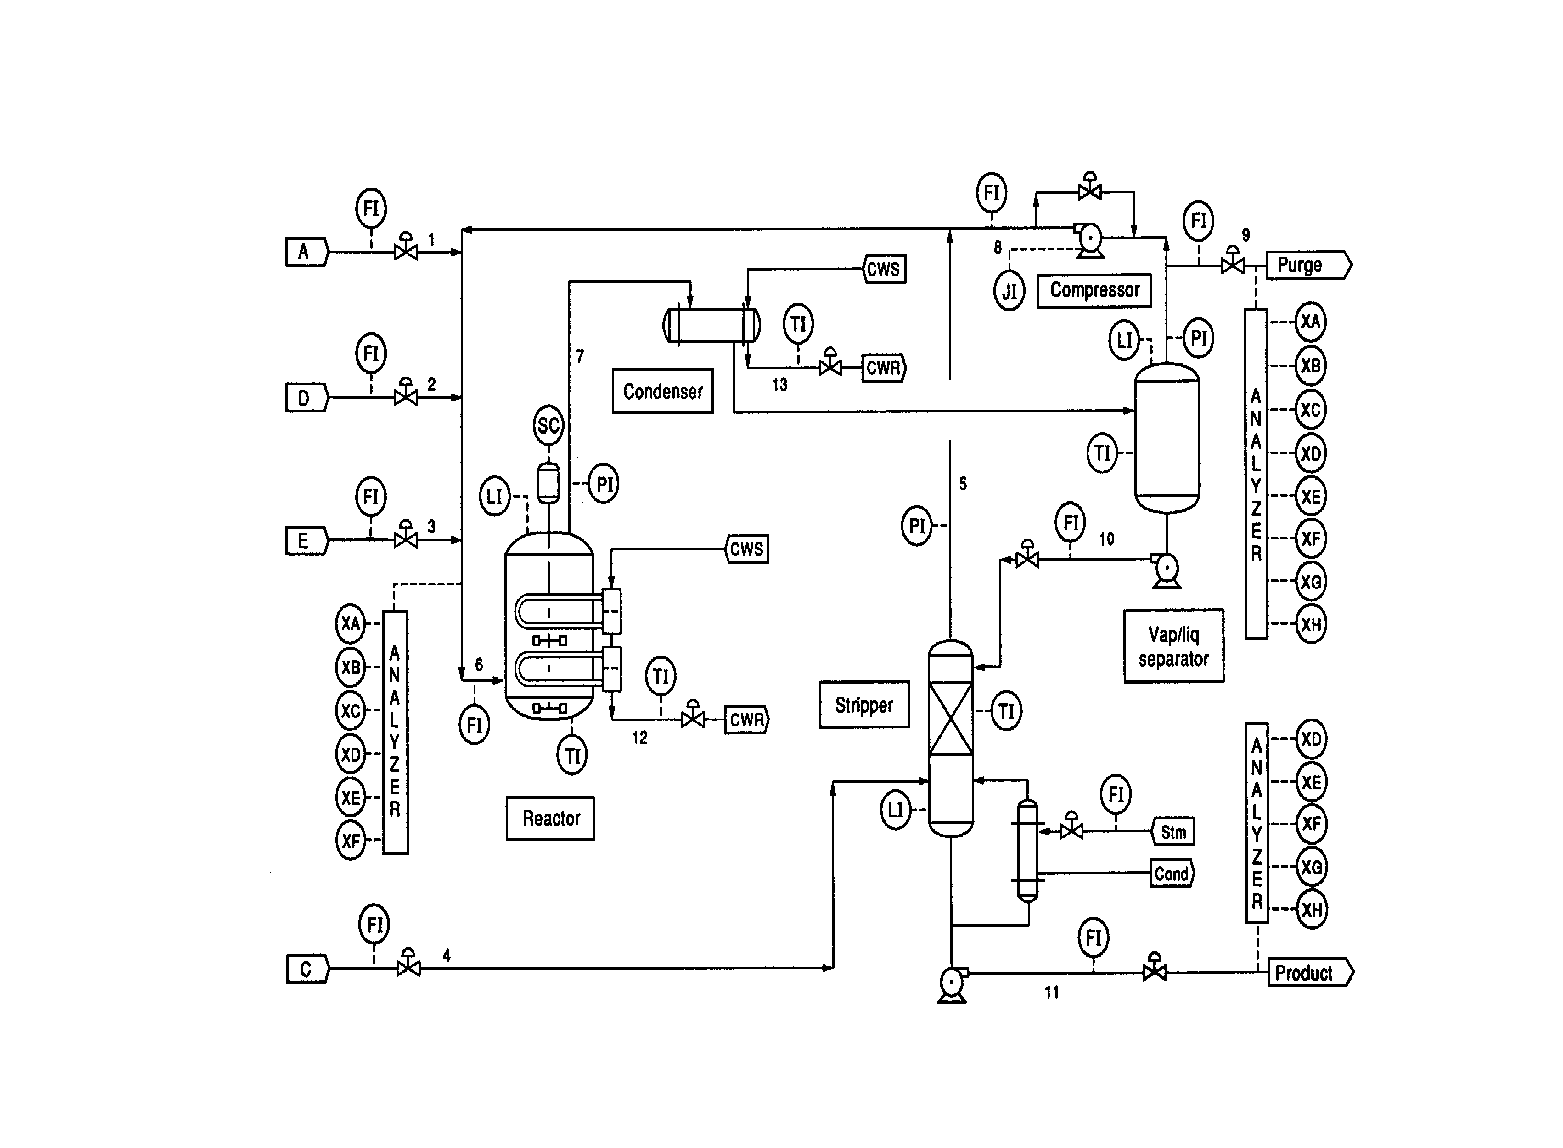
\includegraphics[width=\textwidth]{teflowsheet}
  \caption{Flowsheet for the Tennessee Eastman process~\citep{tenesseeeastman}}
  % TODO: Redraw TE flowsheet properly.
  \label{fig:teprocess}
\end{figure}

Four reactions featuring eight compounds (A through H) take place in the reactor:
\begin{eqnarray}
A(g) + C(g) + D(g) & \rightarrow & G(l) \\
A(g) + C(g) + E(g) & \rightarrow & H(l) \\
A(g) + E(g)        & \rightarrow & F(l) \\
3D(g)              & \rightarrow & 2F(l) 
\label{eq:te-reaction}
\end{eqnarray}

G and H are the first and second products, while F is a byproduct.

\section{CAPE-OPEN}
The CO-lan describes CAPE-OPEN as follows:
\quote{CAPE-OPEN standards are the uniform standards for interfacing
  process modelling software components developed specifically for the
  design and operation of chemical processes. They are based on
  universally recognized software technologies such as COM and
  CORBA. CAPE-OPEN standards are open, multiplatform, uniform and
  available free of charge. They are described in a formal
  documentation set.}

The documentation set comprises the following items:
\subsection{Thermodynamics and Physical Properties Interface Specification}

\subsection{Unit Operations Interface Specification}

\subsection{Chemical Reactions Interface Specification}

\subsection{Methods \& Tools Integrated Guidelines}

\subsection{Optimisation Interface Specification}

\subsection{Parameter Estimation and Data Reconciliation Interface Spec}
This document defines the interfaces required to do parameter estimation and data reconciliation.  The parameter estimation problem is to find the parameters that correspond with the best match between the model and the data, while the data reconciliation problem is to find data that does not correspond to the model.  Both of these activities require a model of the system or the ability to run the model and data from the system.  

\subsection{Partial Differential Algebraic Equations Interface Specification}

\subsection{Petroleum Fractions Interface Specification}

\subsection{Physical Properties Data Bases Interface Specification}

\subsection{Planning and Scheduling Interface Specification}

\subsection{Simulation Context COSE Interface}


\subsection{Identification Common Interface}
\subsection{Parameter Common Interface}
\subsection{Collection Common Interface}
\subsection{Error Common Interface}
\subsection{Persistence Common Interface}
\subsection{Utilities Common Interface}

% Local Variables:
% TeX-master: "thesis"
% End:

